%---------------------------------------------------------------------------
% scrlttr2.tex v0.3. (c) by Juergen Fenn <juergen.fenn@gmx.de>
% Template for a letter to be typeset with scrlttr2.cls from KOMA-Script.
% Latest version of the LaTeX Project Public License is applicable. 
% File may not be modified and redistributed under the same name 
% without the author's prior consent.
%---------------------------------------------------------------------------
\documentclass%%
%---------------------------------------------------------------------------
  [fontsize=12pt,%%          Schriftgroesse
%---------------------------------------------------------------------------
% Satzspiegel
   paper=a4,%%               Papierformat
   enlargefirstpage=on,%%    Erste Seite anders
   firstfoot=off,
   pagenumber=right,%%   Seitenzahl oben mittig
%---------------------------------------------------------------------------
% Layout
   headsepline=off,%%         Linie unter der Seitenzahl
   parskip=half,%%           Abstand zwischen Absaetzen
%---------------------------------------------------------------------------
% Briefkopf und Anschrift
   fromalign=right,%%        Plazierung des Briefkopfs
   fromphone=off,%%           Telefonnummer im Absender
   fromrule=off,%%           Linie im Absender (aftername, afteraddress)
   fromfax=off,%%            Faxnummer
   fromemail=on,%%          Emailadresse
   fromurl=off,%%            Homepage
   fromlogo=off,%%           Firmenlogo
   addrfield=on,%%           Adressfeld fuer Fensterkuverts
   backaddress=on,%%          ...und Absender im Fenster
   subject=beforeopening,%%  Plazierung der Betreffzeile
   locfield=narrow,%%        zusaetzliches Feld fuer Absender
   foldmarks=on,%%           Faltmarken setzen
   numericaldate=off,%%      Datum numerisch ausgeben
   refline=narrow,%%         Geschaeftszeile im Satzspiegel
%---------------------------------------------------------------------------
% Formatierung
   draft=off,%%                Entwurfsmodus
   %backaddress=plain%%        Keine Linie unter Absender
  DIV=12
]{scrlttr2}
%---------------------------------------------------------------------------
\usepackage[english,ngerman]{babel}
\usepackage[T1]{fontenc}
\usepackage[utf8]{inputenc}
\usepackage{url}
\usepackage{lmodern}
\usepackage{csquotes}
\usepackage{pdfpages}
\usepackage{graphics}
\usepackage{pdfpages}
%---------------------------------------------------------------------------
% Fonts
\setkomafont{fromname}{\sffamily}
\setkomafont{fromaddress}{\sffamily}%% statt \small
\setkomafont{pagenumber}{\sffamily}
\setkomafont{subject}{\mdseries}
\setkomafont{backaddress}{\mdseries}
\usepackage{mathptmx}%% Schrift Times
%\usepackage{mathpazo}%% Schrift Palatino
%\setkomafont{fromname}{\LARGE}
%---------------------------------------------------------------------------
\usepackage{lastpage}

\renewcommand*{\pagemark}{{\usekomafont{pagenumber}{%
    \pagename\
    \thepage\ von\ \pageref{LastPage}}}}

\begin{document}
%---------------------------------------------------------------------------
% Briefstil und Position des Briefkopfs
\LoadLetterOption{DIN} %% oder: DINmtext, SN, SNleft, KOMAold.
\makeatletter
\@setplength{firstheadvpos}{20mm}
\@setplength{firstheadwidth}{\paperwidth}
\ifdim \useplength{toaddrhpos}>\z@
  \@addtoplength[-2]{firstheadwidth}{\useplength{toaddrhpos}}
\else
  \@addtoplength[2]{firstheadwidth}{\useplength{toaddrhpos}}
\fi
\@setplength{foldmarkhpos}{6.5mm}
\@addtoplength{firstfootvpos}{-10mm}
\makeatother
%---------------------------------------------------------------------------
% Absender
\setkomavar{fromlogo}{\vspace{-1cm}
\includegraphics[width=4cm]{logo.pdf}}
\setkomavar{backaddress}{ZaPF e.V.\\Max-von-Laue-Str. 1\\60438 Frankfurt / Main}
\setkomavar{fromname}{
\includegraphics[width=2cm]{logo.pdf}\\Zusammenkunft aller Physik-Fachschaften\\c/o ZaPF e.V.\\Goethe Universität Frankfurt\\Raum \_\_.208}
\setkomavar{fromaddress}{Max-von-Laue-Str. 1\\60438 Frankfurt / Main}
%\setkomavar{fromphone}{}
%\renewcommand{\phonename}{Telefon}
\setkomavar{fromemail}{stapf@googlegroups.com}
\setkomavar{backaddressseparator}{ – }
\setkomavar{signature}{Karola Schulz\\Sprecherin des StAPF}
%\setkomavar{frombank}{}
%\setkomavar{location}{\\[8ex]\raggedleft{\footnotesize{\usekomavar{fromaddress}\\
%      Telefon:\ usekomavar{fromphone}}}}%% Neben dem Adressfenster
%---------------------------------------------------------------------------
%\firsthead{Frei gestalteter Briefkopf}
%---------------------------------------------------------------------------
%\firstfoot{}
%---------------------------------------------------------------------------
% Geschaeftszeilenfelder
\setkomavar{place}{Konstanz}
\setkomavar{placeseparator}{, den }
\setkomavar{date}{\today}
%\setkomavar{yourmail}{1. 1. 2003}%% 'Ihr Schreiben...'
%\setkomavar{yourref} {abcdefg}%%    'Ihr Zeichen...'
%\setkomavar{myref}{Test}%%      Unser Zeichen
%\setkomavar{invoice}{123}%% Rechnungsnummer
%\setkomavar{phoneseparator}{}
%---------------------------------------------------------------------------
% Versendungsart
%\setlengthtoplength{\fill}{specialmailindent}
%\setkomavar{specialmail}{Einschreiben mit Rückschein}
%---------------------------------------------------------------------------
% Anlage neu definieren
\renewcommand{\enclname}{Anlagen}
\setkomavar{enclseparator}{: }
%---------------------------------------------------------------------------
% Seitenstil
%\pagestyle{plain}%% keine Header in der Kopfzeile
%---------------------------------------------------------------------------
\newcommand{\massmail}[2]{
\begin{letter}{#1}
%---------------------------------------------------------------------------
% Weitere Optionen
\KOMAoptions{%%
}
%---------------------------------------------------------------------------
\setkomavar{subject}{\textbf{Stellungnahme zur Veröffentlichungspflicht bei Drittmittelforschung}}
%---------------------------------------------------------------------------
\opening{#2}

die Zusammenkunft aller Physikfachschaften hat auf ihrer letzten Tagung am 08.05.20165 die folgende Stellungnahme zur Veröffentlichungspflicht bei Drittmittelforschung verabschiedet.

Für Kommentare und Rückfragen stehen wir Ihnen jeder Zeit zur Verfügung und verbleiben 

Mit freundlichen Grüßen,

\closing{Im Auftrag der ZaPF}
%---------------------------------------------------------------------------
%\ps{PS: 134}
%\encl{}
%\cc{Die Menschheit}
%---------------------------------------------------------------------------

\newpage
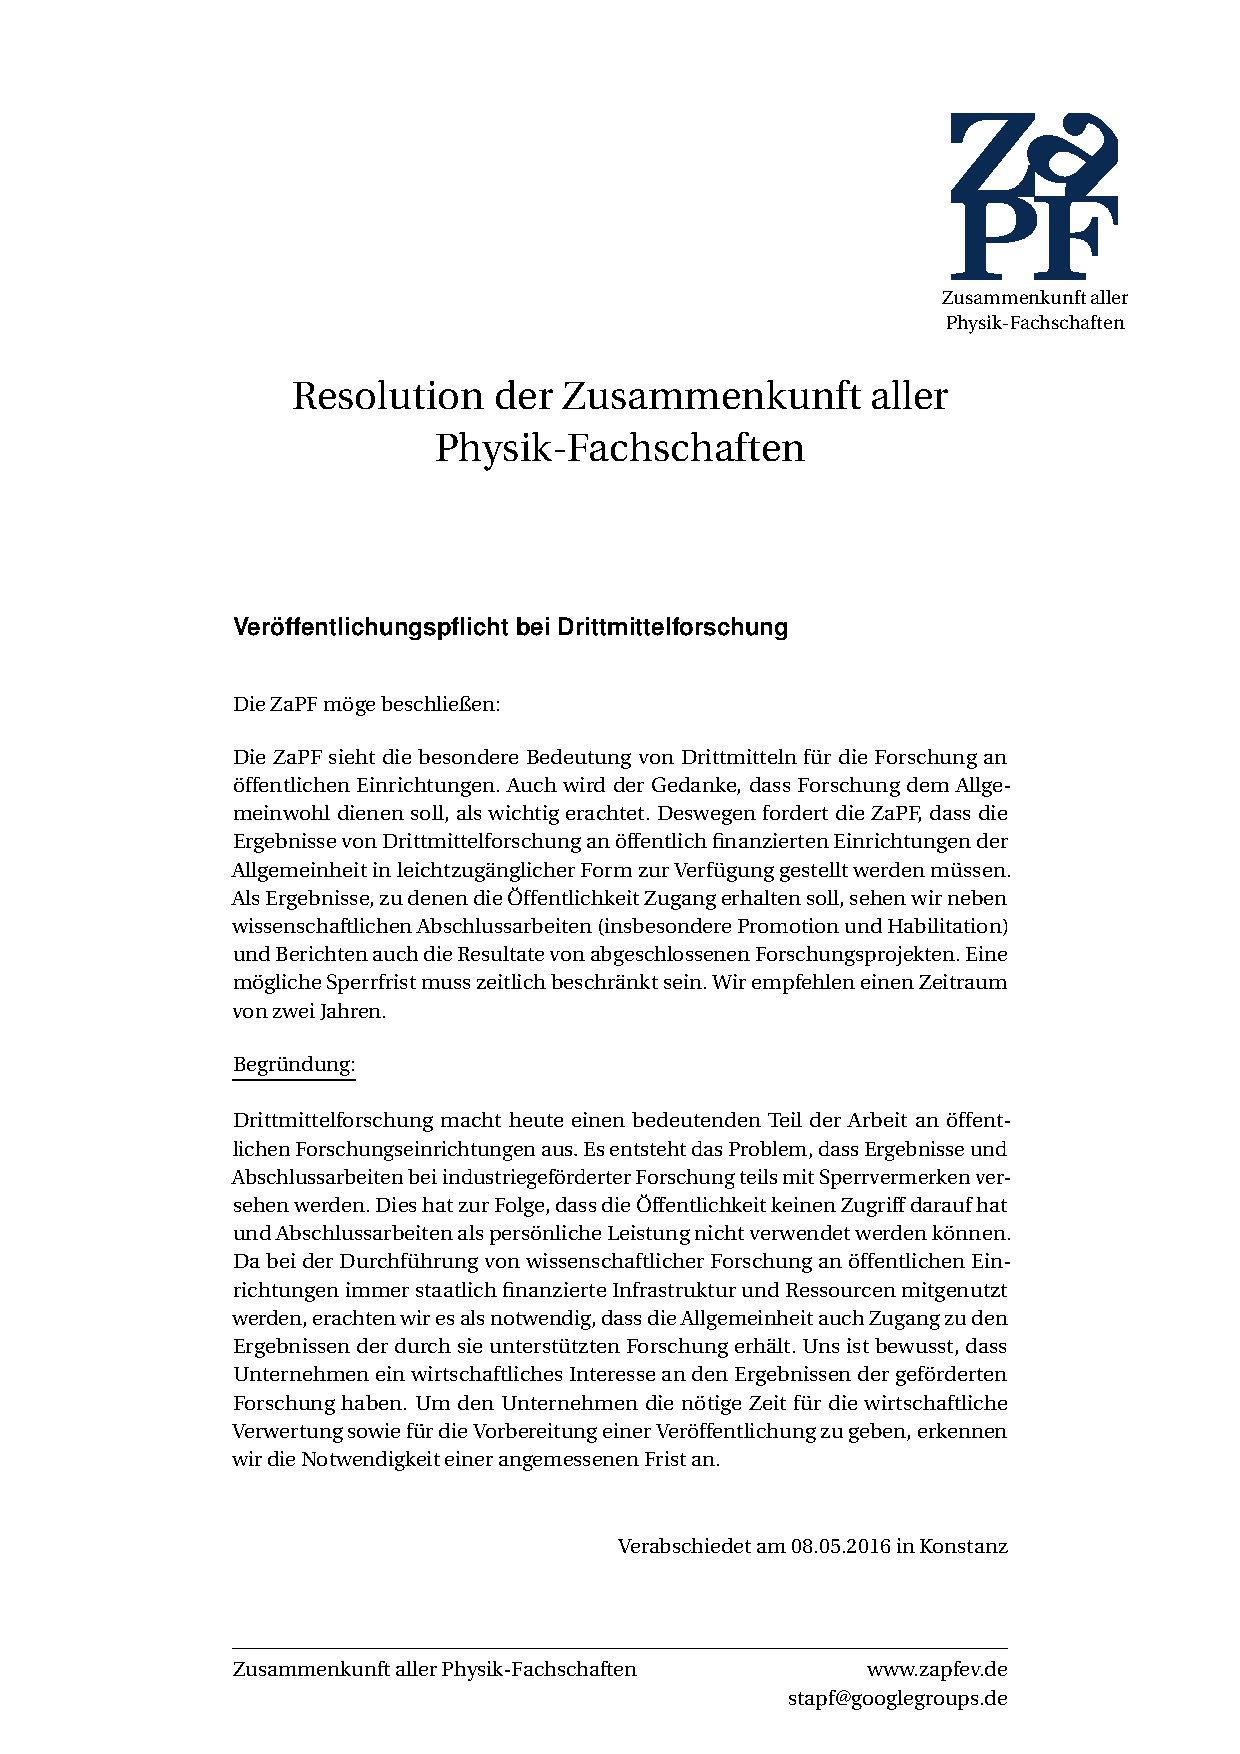
\includepdf[pages=-]{Drittmittel.pdf}

\end{letter}
}
\massmail{Bundesministerium für Bildung und Forschung\\Dienstsitz Berlin\\11055 Berlin}{Sehr geehrte Damen und Herren,}
\massmail{Kultusministerkonferenz\\Postfach 11 03 42\\10833 Berlin}{Sehr geehrte Damen und Herren,}
\massmail{Deutsche Physikalische Gesellschaft\\Hauptstraße 5\\53604 Bad Honnef}{Sehr geehrte Damen und Herren,}
\massmail{Prof. Dr. Gert-Ludwig Ingold\\Sprecher der Konferenz der Fachbereiche Physik\\Institut für Physik\\Universität Augsburg\\86135 Augsburg}{Sehr geehrter Prof. Dr. Ingold,}
\massmail{Hochschulrektorenkonferenz\\Ahrstraße 39\\53175 Bonn}{Sehr geehrte Damen und Herren,}
\massmail{Deutsche Forschungsgemeinschaft\\53170 Bonn}{Sehr geehrte Damen und Herren,}
\massmail{Max-Planck-Gesellschaft\\(mit Bitte um Weiterleitung an die Institute)\\Hofgartenstraße 8\\80539 München}{Sehr geehrte Damen und Herren,}
\massmail{Leibniz-Gemeinschaft\\Sektion D\\(mit Bitte um Weiterleitung an die Institute)\\Chausseestraße 111\\10115 Berlin}{Sehr geehrte Damen und Herren,}
\massmail{Leibniz-Gemeinschaft\\Sektion E\\(mit Bitte um Weiterleitung an die Institute)\\Chausseestraße 111\\10115 Berlin}{Sehr geehrte Damen und Herren,}
\massmail{Fraunhofer-Institut für Angewandte Festkörperphysik IAF\\Tullastraße 72\\79108 Freiburg}{Sehr geehrte Damen und Herren,}
\massmail{Fraunhofer-Institut für Bauphysik IBP\\Fraunhoferstr. 10\\83626 Valley}{Sehr geehrte Damen und Herren,}
\massmail{Fraunhofer-Institut für Bauphysik IBP\\Nobelstr. 12\\70569 Stuttgart}{Sehr geehrte Damen und Herren,}
\massmail{Fraunhofer-Institut für Bauphysik IBP\\Gottschalkstr. 28a\\34127 Kassel}{Sehr geehrte Damen und Herren,}
\massmail{Fraunhofer-Institut für Bauphysik IBP\\c/o Energie Campus, Auf AEG, Bau 16\\Fürther Straße 250\\90429 Nürnberg}{Sehr geehrte Damen und Herren,}
\massmail{Fraunhofer-Zentrum Bautechnik\\c/o Hochschule Rosenheim\\Hochschulstr. 1\\83024 Rosenheim}{Sehr geehrte Damen und Herren,}
\massmail{Fraunhofer-Institut für Kurzzeitdynamik, Ernst-Mach-Institut, EMI\\Eckerstr. 4\\79104 Freiburg}{Sehr geehrte Damen und Herren,}
\massmail{Fraunhofer-Institut für Siliziumtechnologie\\Fraunhoferstraße 1\\D-25524 Itzehoe}{Sehr geehrte Damen und Herren,}
\massmail{Fraunhofer-Institut für Angewandte Polymerforschung IAP\\Geiselbergstraße 69\\14476 Potsdam-Golm\\}{Sehr geehrte Damen und Herren,}
\massmail{Fraunhofer-Institut für Organische Elektronik, Elektronenstrahl- und Plasmatechnik FEP\\Winterbergstraße 28\\01277 Dresden}{Sehr geehrte Damen und Herren,}
\massmail{Fraunhofer-Institut für Optronik, Systemtechnik und Bildauswertung IOSB\\Fraunhoferstraße 1\\76131 Karlsruhe}{Sehr geehrte Damen und Herren,}
\massmail{Fraunhofer-Institut für Optronik, Systemtechnik und Bildauswertung IOSB\\Gutleuthausstraße 1\\76275 Ettlingen}{Sehr geehrte Damen und Herren,}
\massmail{Das Fraunhofer-Institut für Umwelt-, Sicherheits- und Energietechnik UMSICHT\\Osterfelder Str. 3\\46047 Oberhausen}{Sehr geehrte Damen und Herren,}
\massmail{Fraunhofer-Einrichtung für Mikrosysteme und Festkörper-Technologien EMFT\\Hansastrasse 27d\\80686 München}{Sehr geehrte Damen und Herren,}
\massmail{Fraunhofer IWES\\Königstor 59\\34119 Kassel}{Sehr geehrte Damen und Herren,}
\massmail{Fraunhofer-Institut für Windenergie und Energiesystemtechnik\\Institutsteil Nordwest\\Am Seedeich 45\\27572 Bremerhaven}{Sehr geehrte Damen und Herren,}
\massmail{Fraunhofer-Institut für Schicht- und Oberflächentechnik IST\\Bienroder Weg 54 E\\38108 Braunschweig}{Sehr geehrte Damen und Herren,}
\massmail{Fraunhofer-Institut für Elektronische Nanosysteme ENAS\\Technologie-Campus 3\\09126 Chemnitz}{Sehr geehrte Damen und Herren,}
\massmail{Fraunhofer-Institut für Naturwissenschaftlich-Technische Trendanalysen INT\\Postfach 14 91\\53864 Euskirchen}{Sehr geehrte Damen und Herren,}
\massmail{Fraunhofer-Institut für Grenzflächen- und Bioverfahrenstechnik IGB\\Nobelstraße 12\\70569 Stuttgart}{Sehr geehrte Damen und Herren,}
\massmail{Fraunhofer-Institut für Graphische Datenverarbeitung IGD\\Fraunhoferstraße 5\\64283 Darmstadt}{Sehr geehrte Damen und Herren,}
\massmail{Fraunhofer-Institut für Lasertechnik ILT\\Steinbachstr. 15\\52074 Aachen}{Sehr geehrte Damen und Herren,}
\massmail{Fraunhofer-Institut für Photonische Mikrosysteme IPMS\\Maria-Reiche-Str. 2\\01109 Dresden}{Sehr geehrte Damen und Herren,}
\massmail{Fraunhofer-Institut für Solare Energiesysteme ISE\\Heidenhofstr. 2\\79110 Freiburg}{Sehr geehrte Damen und Herren,}
\massmail{Fraunhofer-Institut für Physikalische Messtechnik IPM\\Heidenhofstraße 8\\79110 Freiburg}{Sehr geehrte Damen und Herren,}
\massmail{Fraunhofer Institute for Telecommunications, Heinrich Hertz Institute, HHI\\Einsteinufer 37\\10587 Berlin}{Sehr geehrte Damen und Herren,}
\massmail{Fraunhofer-Institut für Angewandte Optik und Feinmechanik IOF\\Beutenberg Campus\\Albert-Einstein-Str. 7\\07745 Jena}{Sehr geehrte Damen und Herren,}
\massmail{Fraunhofer-Institut für Hochfrequenzphysik und Radartechnik FHR\\Fraunhoferstraße 20\\53343 Wachtberg}{Sehr geehrte Damen und Herren,}
\massmail{Fraunhofer-Institut für Kurzzeitdynamik, Ernst-Mach-Institut, EMI\\Eckerstr. 4\\79104 Freiburg}{Sehr geehrte Damen und Herren,}
\massmail{Helmholtz-Zentrum Berlin für Materialien und Energie\\Hahn-Meitner-Platz 1\\14109 Berlin}{Sehr geehrte Damen und Herren,}
\massmail{Deutsches Elektronen-Synchrotron DESY\\Notkestraße 85\\22607 Hamburg}{Sehr geehrte Damen und Herren,}
\massmail{Helmholtz-Zentrum für Umweltforschung - UFZ\\Permoserstraße 15\\04318 Leipzig}{Sehr geehrte Damen und Herren,}
\massmail{Deutsches Zentrum für Luft - und Raumfahrt (DLR)\\Linder Höhe\\51147 Köln}{Sehr geehrte Damen und Herren,}
\massmail{Forschungszentrum Jülich\\Wilhelm-Johnen-Straße\\52428 Jülich}{Sehr geehrte Damen und Herren,}
\massmail{GSI Helmholtzzentrum für Schwerionenforschung\\Planckstraße 1\\64291 Darmstadt}{Sehr geehrte Damen und Herren,}
\massmail{Helmholtz-Zentrum Dresden-Rossendorf\\Postfach 510119\\01314 Dresden}{Sehr geehrte Damen und Herren,}
\massmail{Karlsruher Institut für Technologie (KIT)\\Kaiserstraße 12\\76131 Karlsruhe}{Sehr geehrte Damen und Herren,}
\massmail{Physikalisch-Technische Bundesanstalt\\Bundesallee 100\\D-38116 Braunschweig}{Sehr geehrte Damen und Herren,}
\massmail{Johannes-Rau-Forschungsgemeinschaft e.V.\\Im \glqq{}Haus der Wissenschaft\grqq{}\\Palmenstraße 16\\40217 Düsseldorf}{Sehr geehrte Damen und Herren,}
%Empfänger: alle deutschsprachigen Hochschulen, alle FSen




%---------------------------------------------------------------------------
\end{document}
%---------------------------------------------------------------------------
